Table files contain information defining the aerodynamic and propulsive forces acting
on a vehicle. Problem files contain the remaining information required to compute a
trajectory, for example a vehicle's initial mass and its flight profile. This
information is combined to integrate the equations of motion, resulting in a
trajectory or flight path.

TAOS can integrate several trajectories simultaneously. Each trajectory represents a
separate vehicle. Information in the table and problem files is used to define the
flight profile for each trajectory or vehicle.

Each trajectory is divided into segments, where each segment can be described with
simple guidance rules. 
\Cref{fig:segmented-flight-paths} shows a maneuvering reentry trajectory. The first
segment is flown ballistically, the second is a constant-angle-of-attack pullout to
level flight, the third is a level turn, and the last is flown ballistically to impact.

\begin{figure}[htbp]
  \centering
  \begin{tikzpicture}[x=1cm,y=1cm,>=Latex,font=\small]
  \draw[thick]
    (0,0) .. controls (1.0,1.2) and (1.8,1.2) .. (2.6,0.8)
    .. controls (3.5,0.3) and (4.6,0.2) .. (5.4,0.35)
    .. controls (6.0,0.5) and (6.3,1.0) .. (5.8,1.25)
    .. controls (5.2,1.55) and (4.9,1.0) .. (5.5,0.8)
    .. controls (6.5,0.45) and (7.2,0.35) .. (7.7,-0.15)
    .. controls (8.0,-0.55) and (8.4,-0.9) .. (8.9,-1.15);
  \fill (0,0) circle (1.5pt);
  \fill (2.6,0.8) circle (1.5pt);
  \fill (5.4,0.35) circle (1.5pt);
  \fill (5.8,1.25) circle (1.5pt);
  \fill (7.7,-0.15) circle (1.5pt);
  \fill (8.9,-1.15) circle (1.5pt);
  \node[below left] at (0,0) {Beginning of trajectory};
  \node[above] at (1.25,1.0) {Segment 1};
  \node[above,align=center] at (3.8,0.95) {Segment 2\\Constant angle-of-attack pullout};
  \node[above,align=center] at (5.9,1.55) {Segment 3\\Level turn};
  \node[below,align=center] at (6.2,0.15) {Segment 4\\Ballistic};
  \node[below right] at (8.9,-1.15) {End of trajectory};
\end{tikzpicture}

  \caption{Segmented Flight Paths.}
  \label{fig:segmented-flight-paths}
\end{figure}

Input data in the problem file describes how each segment is computed: the vehicle
configuration, guidance rules, final conditions, and the next segment to execute.
Segments are joined together continuously to form trajectories.

Problem files have the hierarchical structure shown in
\cref{fig:problem-file-organization}. A problem file contains one or more problems.
Each problem contains information defining one or more trajectories, and each
trajectory definition contains information defining one or more trajectory segments.
A problem can have any number of trajectories, and each trajectory can have any
number of segments. The size of a problem is limited only by available memory and
computer processing speed.

\begin{figure}[htbp]
  \centering
  \resizebox{0.96\linewidth}{!}{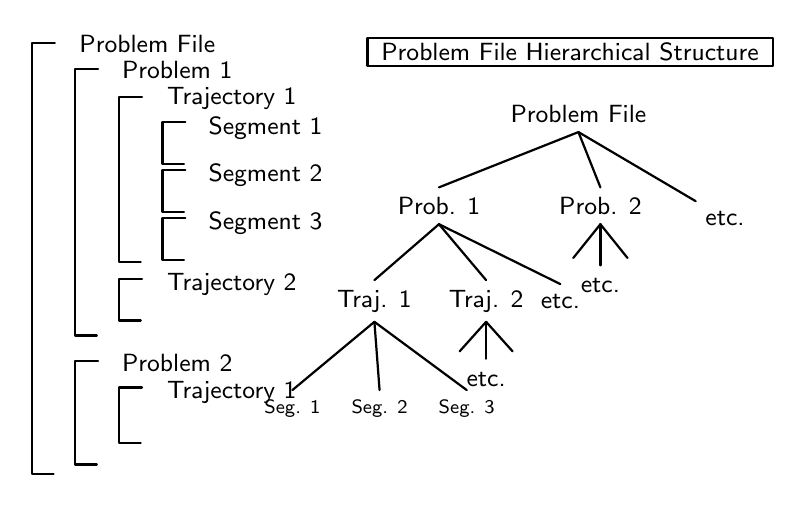
\begin{tikzpicture}[x=0.82cm,y=0.78cm,font=\sffamily\small,line cap=round,line join=round]
  \useasboundingbox (-0.15,0.05) rectangle (11.25,7.45);

  % Left-hand nested-bracket representation from the source figure.
  \draw[line width=0.85pt] (0.25,0.18)--(-0.08,0.18)--(-0.08,7.20)--(0.27,7.20);
  \node[anchor=west] at (0.50,7.18) {Problem File};

  \draw[line width=0.85pt] (0.92,2.44)--(0.58,2.44)--(0.58,6.78)--(0.94,6.78);
  \node[anchor=west] at (1.16,6.76) {Problem 1};

  \draw[line width=0.85pt] (1.60,3.63)--(1.26,3.63)--(1.26,6.32)--(1.62,6.32);
  \node[anchor=west] at (1.86,6.30) {Trajectory 1};

  \draw[line width=0.85pt] (2.27,5.23)--(1.94,5.23)--(1.94,5.91)--(2.29,5.91);
  \draw[line width=0.85pt] (2.27,4.45)--(1.94,4.45)--(1.94,5.13)--(2.29,5.13);
  \draw[line width=0.85pt] (2.27,3.67)--(1.94,3.67)--(1.94,4.35)--(2.29,4.35);
  \node[anchor=west] at (2.50,5.82) {Segment 1};
  \node[anchor=west] at (2.50,5.04) {Segment 2};
  \node[anchor=west] at (2.50,4.26) {Segment 3};

  \draw[line width=0.85pt] (1.60,2.68)--(1.26,2.68)--(1.26,3.36)--(1.62,3.36);
  \node[anchor=west] at (1.86,3.27) {Trajectory 2};

  \draw[line width=0.85pt] (0.92,0.34)--(0.58,0.34)--(0.58,2.02)--(0.94,2.02);
  \node[anchor=west] at (1.16,1.99) {Problem 2};
  \draw[line width=0.85pt] (1.60,0.69)--(1.26,0.69)--(1.26,1.59)--(1.62,1.59);
  \node[anchor=west] at (1.86,1.52) {Trajectory 1};

  % Right-hand tree representation. Nodes are deliberately unboxed to match the
  % historical artwork and branches are separated so labels remain unobstructed.
  \node[draw,line width=0.75pt,inner xsep=5pt,inner ysep=2pt] at (8.25,7.05)
    {Problem File Hierarchical Structure};
  \node (root) at (8.38,6.05) {Problem File};
  \node (p1) at (6.22,4.55) {Prob. 1};
  \node (p2) at (8.72,4.55) {Prob. 2};
  \node (pe) at (10.65,4.35) {etc.};
  \draw[line width=0.8pt] (root.south)--(p1.north);
  \draw[line width=0.8pt] (root.south)--(p2.north);
  \draw[line width=0.8pt] (root.south)--(pe.north west);

  \node (t1) at (5.22,3.00) {Traj. 1};
  \node (t2) at (6.95,3.00) {Traj. 2};
  \node (p1e) at (8.10,3.00) {etc.};
  \draw[line width=0.8pt] (p1.south)--(t1.north);
  \draw[line width=0.8pt] (p1.south)--(t2.north);
  \draw[line width=0.8pt] (p1.south)--(p1e.north);

  \coordinate (p2a) at (8.30,3.70);
  \coordinate (p2b) at (8.72,3.58);
  \coordinate (p2c) at (9.14,3.70);
  \draw[line width=0.8pt] (p2.south)--(p2a);
  \draw[line width=0.8pt] (p2.south)--(p2b);
  \draw[line width=0.8pt] (p2.south)--(p2c);
  \node at (8.72,3.25) {etc.};

  \node[font=\sffamily\scriptsize] (s1) at (3.95,1.25) {Seg. 1};
  \node[font=\sffamily\scriptsize] (s2) at (5.30,1.25) {Seg. 2};
  \node[font=\sffamily\scriptsize] (s3) at (6.65,1.25) {Seg. 3};
  \draw[line width=0.8pt] (t1.south)--(s1.north);
  \draw[line width=0.8pt] (t1.south)--(s2.north);
  \draw[line width=0.8pt] (t1.south)--(s3.north);

  \coordinate (t2a) at (6.54,2.18);
  \coordinate (t2b) at (6.95,2.06);
  \coordinate (t2c) at (7.36,2.18);
  \draw[line width=0.8pt] (t2.south)--(t2a);
  \draw[line width=0.8pt] (t2.south)--(t2b);
  \draw[line width=0.8pt] (t2.south)--(t2c);
  \node at (6.95,1.72) {etc.};
\end{tikzpicture}
}
  \caption{Problem File Organization.}
  \label{fig:problem-file-organization}
\end{figure}

Each trajectory in a problem is identified by a unique trajectory number and name.
TAOS uses the trajectory number internally to identify each trajectory. Both the
trajectory number and name appear in output files. Within a trajectory, each segment
is identified by a unique segment number. Although a descriptive title may be given
for a segment, the title is not used to identify it. Segment numbers must be unique
within a trajectory, but different trajectories may use the same set of segment
numbers.

The following problem file defines a simple trajectory:

\begin{lstlisting}[style=taosmanual]
(pullout)

*title  Example of a maneuvering trajectory
*atmos  standard
*earth  wgs-84

*trajectory 1 rv start on 1

  *initial geodetic
    long=0.0       lat=0.0        psi=90.0       time=0.0
    alt=300000     vel=18000      gama=-30       wt=1000.0

  *print time alt range mach vel gamgd dynprs alpha ca cn

  *segment 1 Ballistic flight
    *aero ca=(rv-ca) cn=(rv-cn)
    *when dynprs>1000 goto 2

  *segment 2 Constant alpha pullout to level flight
    *aero ca=(rv-ca) cn=(rv-cn)
    *fly alpha=10.0
    *when gamgd=0 stop
*end
\end{lstlisting}

This problem file contains one problem, beginning with \tableid{pullout} and ending
with \problemblock{*end}. Although a problem file may contain more than one
problem, it is good practice to place only one problem in each file and run each
problem as a separate task or process. Then a failure in the first problem cannot
prevent other problems from running.

\taossubhead{Data Blocks}

Each set of information in the problem file begins with an asterisk and a name, for
example \problemblock{*title}, \problemblock{*atmos}, or
\problemblock{*trajectory}. These are special names on which TAOS keys to
determine what kind of information follows.

For example, information defining trajectory initial conditions follows the
\problemblock{*initial} keyword:

\begin{lstlisting}[style=taosmanual]
*initial geodetic
  long=0.0       lat=0.0        psi=90.0       time=0.0
  alt=300000     vel=18000      gama=-30       wt=1000.0
\end{lstlisting}

This set of information---everything from the \problemblock{*initial} keyword to
the next \problemblock{*print} keyword---is called a data block. This particular one
is the \problemblock{*initial} data block, and it gives the vehicle's initial state.
Other blocks in the example include the \problemblock{*title} block, which supplies
a problem title; the \problemblock{*atmos} block, which selects the 1976 U.S.
standard atmosphere; and the \problemblock{*earth} block, which selects the WGS-84
earth model. Each data block has a variety of options.

The example defines one trajectory containing two segments. Indentation is used to
show the problem-file structure. The \problemblock{*initial},
\problemblock{*print}, and \problemblock{*segment} blocks are all part of the
\problemblock{*trajectory} block. The \problemblock{*aero},
\problemblock{*fly}, and \problemblock{*when} blocks are part of the
\problemblock{*segment} blocks and may be repeated for each segment. The
indentation follows the hierarchy shown in \cref{fig:problem-file-organization}.

This chapter is organized the same way as the problem file. Each data block is
discussed in a separate subsection, and the subsections are grouped according to the
hierarchy in \cref{fig:problem-file-organization}. 
\Cref{sec:problem-file-format} gives general information about problem-file format;
\cref{sec:segment-data-blocks} describes segment data blocks;
\cref{sec:trajectory-data-blocks} describes trajectory data blocks; and
\cref{sec:problem-data-blocks} describes problem data blocks. The final section,
\cref{sec:problem-examples}, contains example problem files.
